\large
A standard filtered-$x$ least mean square (FXLMS) adaptive algorithm is used to find the counter phase signal of the noise.
The filter coefficients are adapted using the error, measured with microphone (3).

%\vspace{-2mm}
%\begin{equation*}
%	b_j[n+1] = b_j[n] - 2\mu e[n]f[n-j]
%\end{equation*}
 
 
%\begin{centering}
%	\includegraphics[width=\textwidth]{figures/CombinedSystem2.pdf}
%\end{centering}
\resizebox{1\columnwidth}{!}{
	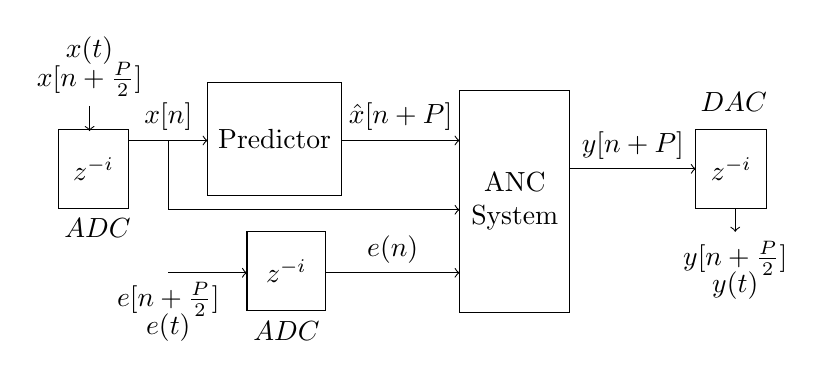
\begin{tikzpicture}
	\draw  (-3.7,1.5) rectangle node {$z^{-i}$} (-4.6,0.5);
	\draw (-4.1,0) node[above]{$ADC$} ;
	\draw (-1.7,-1.3) node[above]{$ADC$} ;
	\draw  (-2.7,2.1) rectangle  node[align=center] {\textrm{Predictor}} (-1,0.66) ;
	
	\draw  (0.5,2) rectangle node[text width=1.5cm,align=center] {\textrm{ANC System}}(1.9,-0.82);
	\draw  (3.5,1.5) rectangle node {$z^{-i}$}(4.4,0.5);
	\draw (3.98,1.6) node[above]{$DAC$} ;
	
	\draw [->](-3.7,1.36)  -- (-2.7,1.36);
	
	
	\draw [->](-1,1.36)  -- node[above]{$\hat{x}[n+P]$}  (0.5,1.36);
	\draw [->](1.9,1) -- node[above]{$y[n+P]$} (3.5,1);
	
	\draw [->](-4.2,1.8) node[above]{$x[n+\frac{P}{2}]$} -- (-4.2,1.48);
	\draw (-4.2,2.2) node[above]{$x(t)$} ;
	\draw [->](4,0.5)-- (4,0.2) node[below]{$y[n+\frac{P}{2}]$} ;
	\draw [->](-3.2,1.36) node[above]{$x[n]$} -- (-3.2,0.48) -- (0.5,0.48);
	\draw (4,-0.78) node[above]{$y(t)$} ;
	\draw  (-1.2,0.2) rectangle node {$z^{-i}$} (-2.2,-0.8);
	
	
	\draw [->](-1.2,-0.32) -- node[above]{$e(n)$} (0.5,-0.32);
	\draw [<-](-2.2,-0.32)-- (-3.2,-0.32) node[below]{$e[n+\frac{P}{2}]$} ;
	\draw (-3.2,-1.32) node[above]{$e(t)$} ;
	\end{tikzpicture}}
The FXLMS is combined with a linear Wiener filter, that allows for prediction of future samples.   
The performance of the predictor can be evaluated by calculating Prediction Gain ($PG$), which is the ratio between the signal and the error variance in dB. A larger $PG$ is better. 
%\vspace{-2mm}
%\begin{equation*}
%	PG = 10 log_{10}\bigg(\frac{\sigma^2_x}{\sigma^2_\varepsilon}\bigg)
%%\end{equation*}

